\documentclass[pdflatex,sn-mathphys-num,iicol]{sn-jnl}

%========================================================
% Packages
%========================================================

\usepackage[utf8]{inputenc}
\usepackage[T5]{fontenc}
\usepackage[vietnamese]{babel}
\usepackage{graphicx}
\usepackage{float}
\usepackage{placeins}
\usepackage{multirow}
\usepackage{amsmath,amssymb,amsfonts}
\usepackage{amsthm}
\usepackage{mathrsfs}
\usepackage{newunicodechar}
\newunicodechar{ℒ}{\mathcal{L}}
\usepackage[title]{appendix}
\usepackage{xcolor}
\usepackage{textcomp}
\usepackage{manyfoot}
\usepackage{booktabs}
\usepackage{algorithm}
\usepackage{algorithmicx}
\usepackage{algpseudocode}
\usepackage{listings}
\usepackage{url}

%========================================================
% Theorem styles
%========================================================
\theoremstyle{thmstyleone}
\newtheorem{theorem}{Theorem}

\theoremstyle{thmstyletwo}
\newtheorem{example}{Example}
\newtheorem{remark}{Remark}

\theoremstyle{thmstylethree}
\newtheorem{definition}{Definition}

\raggedbottom

%========================================================
% Document
%========================================================
\begin{document}

%========================================================
% Title
%========================================================
\title[Development of an Aspect-Based Review QA Chatbot for Hotel Services]
{Development of an Aspect-Based Review QA Chatbot for Hotel Services}

%========================================================
% Authors
%========================================================
\author*[1]{
\fnm{Nguyen Pham Minh} \sur{Triet}
}

\author[1]{
\fnm{Nguyen Hoang Duy} \sur{Tien}
}

\author[1]{
\fnm{Nguyen Bui Anh} \sur{Duy}
}

\affil*[1]{
\orgname{FPT University},
\orgaddress{
\city{Ho Chi Minh City},
\country{Vietnam}
}
\textit{Lecturer: Bui Danh Huong}
}

%========================================================
% Abstract
%========================================================

\abstract{
...
}


%========================================================
% Keywords
%========================================================
\keywords{
...
}

\maketitle

%========================================================
% 1. INTRODUCTION
%========================================================
\section{Introduction}
\label{sec:introduction}

\subsection{Background and Motivation}
\label{subsec:background}
Trong lĩnh vực dịch vụ du lịch việc đón nhận các đánh giá trực tuyến của khách hàng đóng vai trò quan trọng trong việc cung cấp thông tin về chất lượng sản phẩm và dịch vụ, Tuy nhiên, các điểm đánh giá chỉ phản ảnh được một số mức độ hài lòng tổng quát nhưng chưa gaiir thích được nguyên nhân khiến phần lớn khách hàng đưa ra đánh giá như vậy. Theo paper~\cite{namee2023hybrid}, “rating scores alone are not sufficient to undertake quality improvement of goods or understand the reasons for customer retention”~\cite{namee2023hybrid}. Bên cạnh đó, việc phân tích bằng những phương pháp thủ công sẽ bị hạn chế về công sức (nhân sự) hay thời gian sẽ dẫn đến một vấn đề, đó là sự trên lệch. Những hạn chế này sẽ dễ dàng cho thấy được về sự cần thiết của các phương pháp công khai về thông tin chi tiết từ dữ liệu đánh giái trực tuyến.

Phân tích theo cảm xúc của từng khía cạnh (Aspect-Based Sentiment Analysis – ABSA) là một hướng tiếp cận giúp xác định rỏ cảm xúc của khách hàng theo từng khía cạnh cụ thể. Paper~\cite{namee2023hybrid} chỉ ra việc phân tích cảm xúc nếu chỉ theo cấp độ tài liệu thì chỉ có thể đánh giá được phần nào, chứ chưa chắc sẽ đánh giá chính xác việc một người khách có thật sự thích hay k thích một sản phẩm, dịch vụ; trong đó, nêu việc phân tích theo đúng khía cạnh có thể làm rõ cảm xúc gắn với từng cử chỉ hay đặc điểm cụ thể. Đối với lĩnh vực khách sạn, phần lớn các khía cạnh sẽ được chú ý bảo gồm chất lượng phục vụ, sự thoải mái, độ sạch sẽ, vị trí và thái độ của nhân viên~\cite{bimaputra2023aspect} "The selected aspects refer to the aspects that the hotel provides to its customers in creating its own competitiveness, broadly speaking these aspects such as hotel safety, service, comfort, attitude of hotel staff and cleanliness of the hotel environment."~\cite{bimaputra2023aspect}. Việc dựa trên các khía cạnh đó để đánh giá và đưa ra nhận xét về chất lượng dịch vụ vì vậy việc cung cấp thông tin chi tiết sẽ tốt hơn rất nhiều cho trải nghiệm của người khách hàng đối với khách sạn hay các dịch vụ lưu trú.

Xuất phát từ những hạn chế trên, đề tại này hướng đế để có thể xây dưng một hệ thống chatbot hỏi đáp (Question Answering -  QA Chatbot) cho người tiêu dùng, để có thể tăng phần nào trải nghiệm, dựa trên việc đánh giá và phân tích đa khía cạnh. Hệ thống thường hướng đến người tiêu dùng nên giao diện sẽ phần nào dễ dùng cũng như truy vấn thống tin bằng ngôn ngữ tự nhiên để giúp dễ dàng đưa ra câu trả lời phù hợp cho họ, thay vì phải tự tìm và xem từng đánh giá trên mạng xã hội. Qua đó, đề tài này sẽ khai thác ưu điểm của phân tích cảm úc theo khía cạnh để cố thể hổ trợ người dùng có thể tiếp cận được thông tin uy tín và chất lượng khách sạn một cách thuận tiện và có trong tâm hơn là việc chỉ trả lời qua loa.


\subsection{Problem Statement and Research Gap}
\label{subsec:problem}
Mặc dù việc phải liên tục phân tích theo các khía cạnh cảm xúc của con người (Aspect-Based Sentiment Analysis – ABSA) để có thể giúp khai thác ý kiến khách háng chi tiết hơn, nên việc có thể đưa ra đánh giá cũng như là xây dựng được một hệ thống hỏi đáp sẽ phải chịu nhiều thách thức lớn.

\textbf{Thứ nhất, về mâu thuẫn cảm xúc nội tai (Conflicting Sentiments).} Một đánh giá sẽ có thể có nhiều mặt cảm xúc trong đó như việc có thể đưa ra đánh giá tích cực và đồng thời cũng có thể có một số tiêu cực đối với một số khía cạnh khác nhau, chẳng hạn như khen phòng sạch nhưng mà chất lượng dịch vụ rất tệ hay nhân viên có thái độ không tốt. Việc có nhiều cảm xúc trong một bình luận sẽ gây khó khăn, cũng như là rào cản rất lớn trong quá trình học hỏi của chatbot, khi phải liên tục đánh giá xem khia cạnh nào bị đánh giá xấu.

\textbf{Thứ hai, về vấn dề thời gian (Time Weighting)}. Khi mà có quá nhiều nhữ đánh giá cụ thể, việc phải lựa trọn xem chất lượng của đánh giá tại thời điểm đó có đúng không. Phần lớn cách đánh giá sẽ sau này sẽ cho ra kết quả đúng so với các đánh giá cũ tại cùng một thời điểm. Vì vậy hệ thống sẽ ưu tiên lựa chọn những cái gần tại thời điểm đó nhất. Ví dụ như việc ta có hai đánh giá như sao, 01/01/2019 cho là 2 sao trên thang điểm chấm, trong khi đánh giá gần đây nhất là 02/10/2026 sẽ cho kết quả là 5 sao trên thang điểm và đưa ra những đánh giá cụ thể hơn. Dựa vào đó kết quả đánh giá sao này sẽ cho thấy dịch vụ cũng như là chất lượng đã thay đổi nhiều hơn sau này. vì vậy các giá trị mang tính minh hoạ cho cơ chế ưu tiên hơn khi lựa chọn thông tin mới nhất.

\textbf{Cuối cùng, hiểu ngữ cảnh và liên kết các câu lệnh trong hội thoại (Context Understanding and Conversational Continuity)}. Chatbot cần hiểu mối liên hệ giữa các câu hỏi liên tiếp nhau và ghi nhận lại những thông tin từ các cuộc hội thoại đó. Nếu không thể duy trì được ngũ cảnh, hệ thông sẽ đưa ra những câu trả lời không chính xác theo yêu cầu của người dùng.


\subsection{Proposed Framework: CRAM-ABSA}
\label{subsec:proposed_framework}
Nhằm giải quyết triệt để các hạn chế về xung đột cảm xúc đa khía cạnh, suy diễn sai lệch do dữ liệu phân bố lệch và hiện tượng lẫn bằng chứng đã nêu tại Mục~\ref{subsec:problem}, chúng tôi đề xuất khung kiến trúc học đồng thời \textbf{CRAM-ABSA} (\textit{Cross-Aspect Rationale Alignment Model for Aspect-Based Sentiment Analysis}). Bản chất của các bài đánh giá khách sạn trực tuyến luôn tồn tại sự phân cực phức tạp; như nghiên cứu của Tran và Tran~\cite{tran2026aspect} đã nhận định: ``\textit{Conventional sentiment analysis techniques, which typically operate at document or sentence levels, often fail to capture the nuanced opinions embedded within specific aspects... a single review might praise the cleanliness of a hotel while critiquing its location, necessitating a more granular analytical framework to discern these multifaceted sentiments accurately}'' ~\cite{tran2026aspect}. Hơn nữa, việc mô hình hóa sự phụ thuộc tương hỗ giữa các khía cạnh là yếu tố quyết định bởi tính giao thoa ngữ nghĩa tự nhiên trong đánh giá dịch vụ. CRAM-ABSA được thiết kế như một hệ thống liên kết thống nhất gồm bốn khối chức năng chính:

\begin{enumerate}
    \item \textbf{Khối mã hóa ngữ cảnh và dung hợp siêu dữ liệu (Context \& Metadata Fusion Encoder):} Sử dụng mô hình Transformer tiền huấn luyện (BERT/BART backbone) kết hợp mạng chiếu phi tuyến (Dense Projection) để tích hợp các đặc trưng phi văn bản (trọng số thời gian đánh giá, xếp hạng sao khách sạn) vào biểu diễn ngữ nghĩa ẩn. Thiết kế này kế thừa định hướng từ nghiên cứu của Bruni và cộng sự~\cite{bruni2025amaqa}, khắc phục hạn chế lớn của các mô hình hỏi đáp thông thường: ``\textit{Retrieval-augmented generation (RAG) systems are widely used in question-answering (QA) tasks, but current benchmarks lack metadata integration, limiting their effectiveness in domain-specific scenarios}''~\cite{bruni2025amaqa}.
    
    \item \textbf{Module sinh bằng chứng định hướng khía cạnh (Aspect Rationale Generator):} Khởi tạo mặt nạ mềm $m_a \in [0, 1]^L$ nhằm xác định chính xác các đoạn căn cứ (rationale) cho từng khía cạnh $a$. Nhằm loại bỏ hiện tượng rò rỉ bằng chứng liên khía cạnh (cross-aspect leakage), mô hình tích hợp hàm mất mát phạt chồng lấn phân đoạn ($\mathcal{L}_{\text{overlap}} = \lambda_2 \sum_{a \neq b} \langle m_a, m_b \rangle$), ràng buộc các vùng bằng chứng giữa các khía cạnh khác nhau phải độc lập và không bị lấn chiếm.
    
    \item \textbf{Đầu hồi quy thứ bậc và phân loại cảm xúc (Ordinal Rating \& Sentiment Heads):} Thay vì đơn giản hóa bài toán về phân loại nhị phân, CRAM-ABSA dự đoán trực tiếp mức độ hài lòng trên thang điểm 5 sao thông qua hàm mất mát thứ bậc CORN (Conditional Ordinal Regression for Neural Networks) kết hợp trọng số phạt nghịch đảo tần suất lớp $\omega(y_a)$, phản ánh đúng trật tự khoảng cách mức sao và xử lý hiệu quả hiện tượng mất cân bằng dữ liệu cực đoan.
    
    \item \textbf{Bộ giải mã hội thoại phục vụ Chatbot QA (Generative Decoder):} Tiếp nhận các biểu diễn văn bản đã được tăng cường trọng số từ bằng chứng khía cạnh ($x \odot (1 + m_a)$) để tự động sinh câu trả lời tự nhiên, giàu thông tin và minh bạch căn cứ cho người dùng trong từng phiên truy vấn.
\end{enumerate}
\subsection{Research Questions}
\label{subsec:research_questions}

This research addresses five research questions:

\begin{enumerate}


    \item \textbf{RQ1: Khi chuyển từ bài toán phân loại nhị phân 2 lớp (Tốt/Xấu) sang thang điểm 5 mức sao thực tế, độ chính xác khi tìm đoạn bằng chứng (rationale) và đánh giá cảm xúc theo từng khía cạnh giảm bao nhiêu, và sự sụt giảm này có tập trung chủ yếu ở các mức đánh giá trung gian (2 đến 4 sao) hay không?}
    
    Đa số các bài báo trước đây thường gộp điểm đánh giá thành 2 nhóm đơn giản: "Khen" và "Chê". Thực tế, khách sạn chấm điểm từ 1 đến 5 sao (rất
    khó phân biệt giữa 3 sao và 4 sao). RQ1 chứng minh rằng bài toán 5 sao thực tế khó hơn rất nhiều so với bài toán nhị phân, đặc biệt ở các review có mức điểm trung bình.
    
    --> Điểm Token-F1 của đoạn bằng chứng, Macro-F1 của phân loại cảm xúc tách biệt theo từng mức từ 1 đến 5 sao.


    \item \textbf{RQ2: Cơ chế phạt chồng lấn phân đoạn ($\mathcal{L}_{\text{overlap}}$) kết hợp hàm mất mát thứ bậc (CORN Loss) trong mô hình CRAM-ABSA có giúp loại bỏ hiện tượng 'lẫn bằng chứng' giữa các khía cạnh và giảm sai lệch dự đoán điểm sao mà không làm suy giảm chất lượng trích xuất câu văn hay không?}
    
    Trong một bài đánh giá, khách thường viết: "Phòng rất sạch nhưng nhân viên phục vụ chậm chạp". Mô hình thông thường hay bị "lẫn", lấy câu khen phòng sạch để làm căn cứ chấm điểm cho dịch vụ nhân viên - Aspect: Services. 
    
    --> Tỷ lệ chồng lấn/lẫn token giữa các khía cạnh (Leakage Rate), sai số tuyệt đối trung bình theo thứ tự (Macro-MAE), và Token-F1 qua thí nghiệm bóc tách thành phần (Ablation Study)
    



    \item \textbf{RQ3: Việc tích hợp bằng chứng khía cạnh từ CRAM-ABSA cùng cơ chế ưu tiên đánh giá mới theo thời gian (Time-weighting) giúp Chatbot cải thiện độ chính xác và tính thuyết phục của câu trả lời như thế nào so với các mô hình hỏi đáp truyền thống trên bộ benchmark thực tế?}

    Người dùng hỏi Chatbot: "Dạo này bữa sáng khách sạn thế nào?". Chatbot cần ưu tiên các review gần đây (vì chất lượng năm 2026 có thể đã khác năm 2019) và phải trích dẫn đúng đoạn nhận xét về bữa sáng để trả lời. RQ3 đánh giá xem chatbot được xây dựng có trả lời đúng trọng tâm và đáng tin cậy hơn chatbot thông thường trên bộ 60 câu hỏi thử nghiệm hay không.
    
    --> Điểm ROUGE-L / Token-F1 của câu trả lời sinh ra, tỷ lệ câu trả lời truy xuất đúng bằng chứng khía cạnh (Aspect Retrieval Accuracy) trên bộ QA Benchmark qa-verified.json.


    
\end{enumerate}


\subsection{Key Contributions}
\label{subsec:key_contributions}

The key contributions of this research as follows:
\begin{itemize}

    \item \textbf{a. Bộ benchmark gopf 60 câu hỏi QA thực nghiệm dành cho chatbot:} 
    
    Chúng tôi xây dựng bộ benchmark gồm 60 câu hỏi- đáo dùng để đánh giá chatbot hỏi đáp dựa trên review thật từ tất cả khách sạn có đánh giá trên thị trường. Bộ câu hỏi nhằm vào các khả năng truy xuất đúng bằng chứng theo cạnh và tổng hợp ý kiên từ nhiều đánh giá, thay vì chỉ đo độ  chính xác được phân loại theo từng cảm xúc của con người. Đây là thước đo gần với tính huống sử dụng thực tế hơn các chỉ số ABSA được công số trên truyền thông.

    \item \textbf{b. Bộ giao diện UI được thử nghiệm và ablation study có đối chứng chặt chẽ trên dữ liệu khách sạn:}
    
    Chúng tôi thiết giao diện thử nghiệm để người dùng có thể đặt câu hỏi và xem được câu trả lời kèm theo hình ảnh cũng như là bằng chứng góc về những đoạn đánh giá về khách sạn đó. Song song đó, ablation study được thực hiện trên cùng bộ dữ liệu của khách sạn, với các điều kiện được kiểm soát. Nghiên cứu so sánh và đánh giá về sự khác biệt giữa bài toán phân loại nhị phân và phân loại thứ bậc theo 5 mức như (RQ1), đồng thời phải đưa ra và phân tích được những ảnh hướng riêng biệt của từng thành phần của từng hàm mất mát, bao gồm Ordinal Loss (CORN) và cơ chế phạt chồng lấn (RQ3), nhằm làm rõ đóng góp của từng thành phần đối với hiệu quả mô hình.


    \item \textbf{c. Framework học đồng thời CRAM-ABSA giải quyết việc xung đột cảm xúc trên từng bình luận của từng khách sạn:}
    
     Một bài đánh giá thường khen khía cạnh này những cũng có thể sẽ có chê những khía cạnh khác. Phân tích dữ liệu cho thấy tình huống này khá phổ biến, ví dụ có hơn 640 các review của 1 khách sạn thường trong đó sẽ bao gôm khen, chê hay có thể có cả 2 trong một bài đánh giá. Vì vậy CRAM-ABSA học đồng thời việc phải xác định đoạn bằng chứng (rationale) và dự đoán cảm xúc theo từng khía cạnh. Mục tiêu là giảm hiện tượng bằng chứng của khía cạnh này "lẫn" sang khía cạch khác (RQ2,RQ3), mà không làm giảm các biến đánh giá của F1.
\end{itemize}



%========================================================
% 2. Research Method
%========================================================
\section{Research Method}
\label{sec:researchmethod}

\subsection{Thiết kế nghiên cứu - Research Pipeline}
\label{subsec:researchpipeline}

...

\subsection{Dữ liệu \& Thu thập - Data Collecting}
\label{subsec:datacollecting}

a. Nguồn dữ liệu.

Chúng tôi sử dụng bộ dữ liệu review khách sạn tiếng Anh từ TripAdvisor, lưu trong tệp TripAdvisor\_EN.json. Bộ dữ liệu gồm 9.9990 bài đánh giá từ các khách sạn trải dài khắp Việt Nam với  hơn 54.326 chú thích từ đa khía cạnh (trung bình có hơn 5 chú thích cho mỗi bài đánh giá). Dữ liệu được gắn nhãn sẵn, nên chúng tôi tận dụng những gì đã có.

b. Cách gắn nhãn của dữ liệu gốc.

Tệp JSON có định dạng xuất từ công cụ dán nhãn Label Studio. mỗi bản ghi gồm ba phần:

- Văn bản review (data.text).
- Siêu dữ liệu(meta\_info): mã tham chiếu, tên địa chỉ khách sạn, ví trí, hạng sao khách sạn, điểm đánh của khách(score, từu 1 đến 5 sao), ngày, năm, tháng.
- Chú thích( annotations): mỗi bài có một danh sách kết quả gán nhãn ở mức đoạn văn (span-level).

Mỗi đoạn bằng chúng được gắn nhãn qua hai bước, liên kết với nhau bằng cùng một mã ID:

c. Thống kê tổng quan và phân tích EDA
Phân bố điểm đánh giá. Dữ liệu lệch mạnh về phía tích cực:5 sao chiếm 71,55\% và nếu gộp thành 2 lớp thì nhãn dán tích cực chiểm 89,33\%. Nhóm1 đến 3 sao chỉ có khoản hơn 1.000 bài, tức là khoản 10,6\%. Sự mất cân bằng này là thách thức chính khi phân biệt các mức độ đánh trung gian trong các khoản từ (2 đến 4 sao). 

Độ dài văn bản. Mỗi bài review dài trung bình 350,7 ký tử (82,1 ký tự), trung vị 398 ký tự (72 từ). Độ dài dao động từ 177 đến 847 ký tự, tương ứng khoảng từ 30 đến 150 từ. phạm vi hẹp này cho thấy dữ liệu gốc có vẻ đã được chọn lọc rất kỷ từ trước thèo độ dài, nên văn bản phù hợp với giới hạn đầu vào của các mô hình ngôn ngũ huấn luyệnp.

\begin{figure}
    \centering
    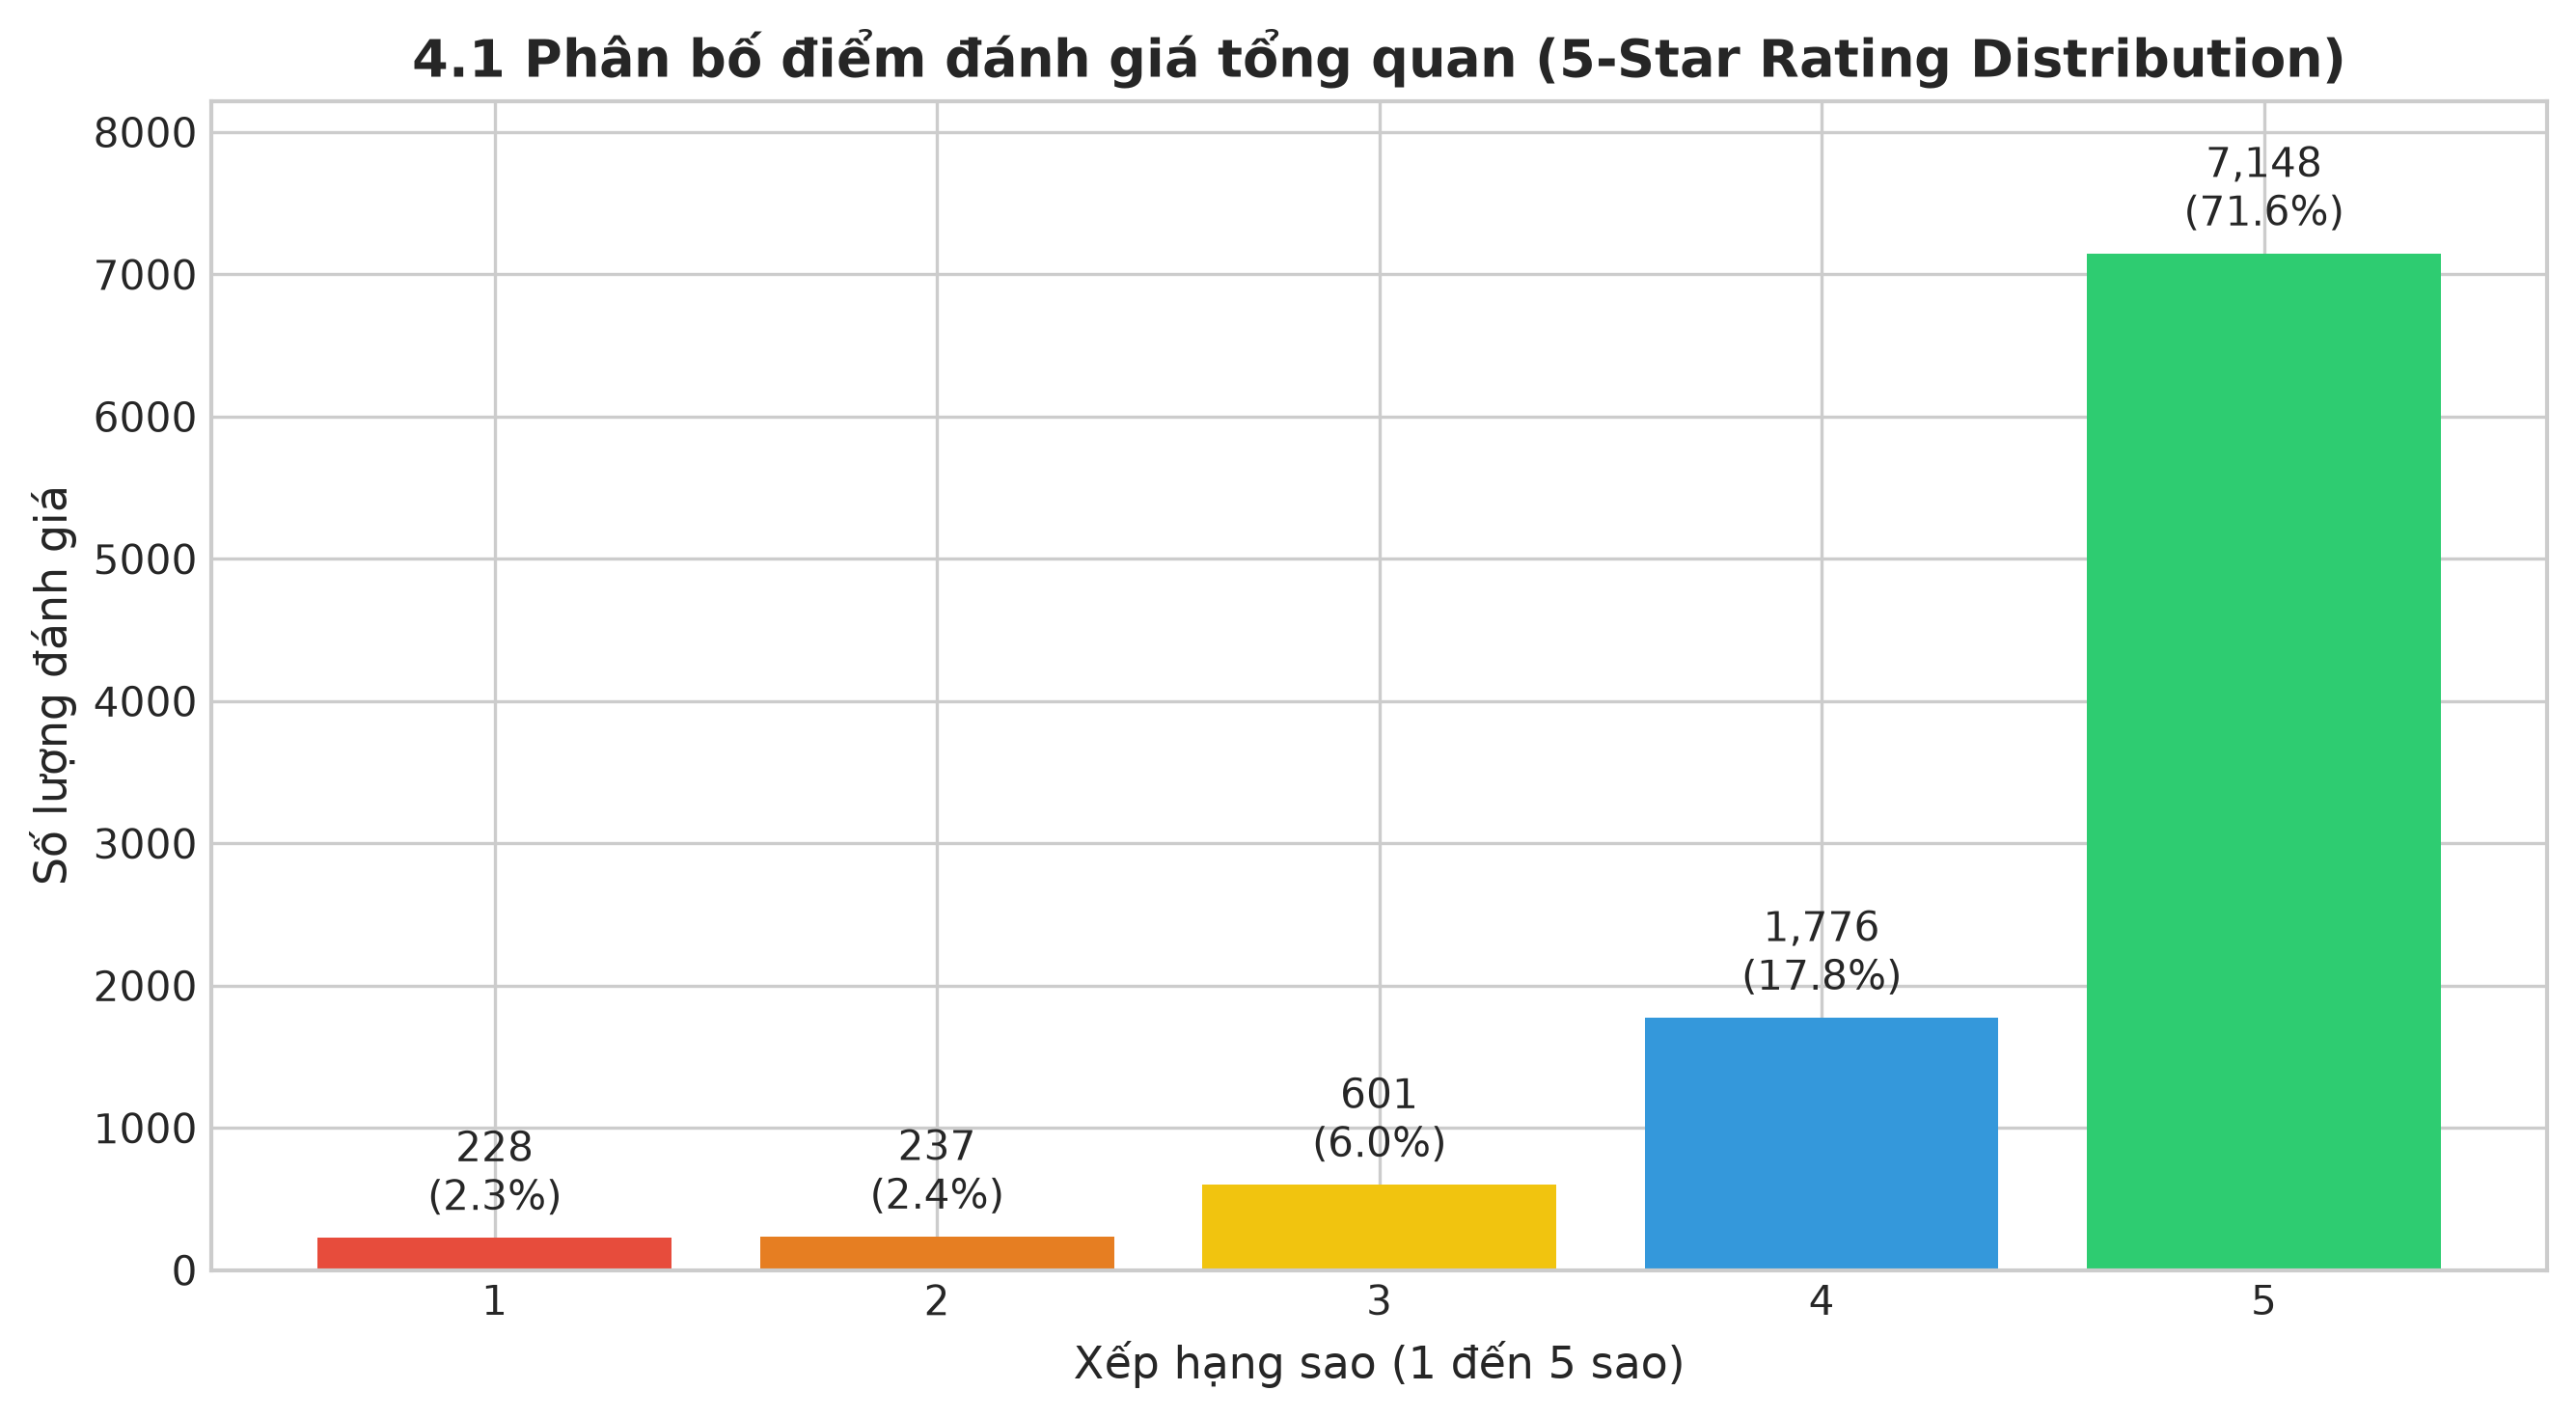
\includegraphics[width=0.8\linewidth]{chart_img/41_overall_rating_distribution.png}
    \caption{Phân bố điểm đánh giá.}
    \label{fig:placeholder}
\end{figure}

\subsection{Tiền xử lý - Data Preprocessing (EDA)}
\label{subsec:datapreprocessing}

...


\subsection{Phát biểu bài toán - Problem Statement}
\label{subsec:problemstatement}

Trong nghiên cứu này, chúng tôi tập trung xây dựng một hệ thống phân tích đánh giá khách sạn theo từng khía cạnh và sử dụng kết quả phân tích để hỗ trợ chatbot trả lời câu hỏi của người dùng. Phương pháp phân tích cảm xúc theo khía cạnh (Aspect-Based Sentiment Analysis -- ABSA) đã được chứng minh là hướng tiếp cận cần thiết khi các phương thức khảo sát truyền thống không còn đáp ứng được lượng phản hồi trực tuyến khổng lồ; như Nawawi và cộng sự~\cite{nawawi2024exploring} đã chỉ ra: ``\textit{Traditional feedback methods like surveys often fail to capture the nuanced and real-time experiences of tourists... This study proposes integrating aspect-based sentiment analysis with zero-shot learning to analyze online tourist reviews effectively without requiring extensive annotated datasets}''~\cite{nawawi2024exploring}. Bên cạnh đó, việc áp dụng các phương pháp lai kết hợp giữa khai phá ý kiến và xử lý ngôn ngữ tự nhiên cũng được Yu và cộng sự~\cite{yu2024dynamic} nhấn mạnh nhằm mở rộng quy mô phân tích đa thuộc tính dịch vụ: ``\textit{This study compared and analysed the consumer demands of hotels in different cities via a dynamic perspective, and used hybrid methods to improve the granularity of the analysis}''~\cite{yu2024dynamic}. Đồng thời, việc phân tích định lượng tương quan giữa các chủ đề khía cạnh trong văn bản nhận xét với điểm số đánh giá thực tế của khách hàng đã khẳng định tính vượt trội so với việc chỉ nhìn nhận cảm xúc chung, đúng như nhận định của Nakamura và Oomiya~\cite{nakamura2021applying}: ``\textit{the relationships between topics and evaluations, which are quantified to consider future guidelines and services}''~\cite{nakamura2021applying}.

Từ đó, nghiên cứu hướng đến việc giải quyết ba nhiệm vụ chính: trích xuất đoạn văn bản làm bằng chứng cho từng khía cạnh, xác định cảm xúc tương ứng và dự đoán điểm đánh giá tổng thể. Các kết quả này tiếp tục được sử dụng để hỗ trợ chatbot tìm kiếm thông tin và trả lời câu hỏi dựa trên những đánh giá thực tế của khách hàng.

\subsubsection{Định nghĩa bài toán}

Đầu vào của hệ thống là nội dung đánh giá khách sạn cùng với những thông tin liên quan có sẵn, chẳng hạn như tên khách sạn, điểm đánh giá và thời gian đăng bài. Cấu trúc dữ liệu này kế thừa định dạng chuẩn hóa trong nghiên cứu phản hồi trực tuyến của Nakamura và Oomiya~\cite{nakamura2021applying}: ``\textit{Each data point is composed of each contributor's review text, assessment scores, and the date on which the review was published}''~\cite{nakamura2021applying}, trong đó các tác giả xác định rõ các thành phần đánh giá bao gồm: ``\textit{assessment items such as `overall,' `cleanliness,' `service and staff,' `amenities' and `properly conditioned.' Their items are 5 points of Likert scales}''~\cite{nakamura2021applying}. Từ những thông tin này, hệ thống cần xác định các khía cạnh được đề cập, tìm những đoạn văn bản thể hiện nhận xét của khách hàng và dự đoán cảm xúc tương ứng. Ngoài ra, nghiên cứu còn xem xét nhiệm vụ dự đoán điểm đánh giá tổng thể trên thang từ 1 đến 5 sao.

Có thể biểu diễn đầu vào của bài toán như sau:

\[
X = (R, M)
\]

Trong đó, $R$ là nội dung bài đánh giá và $M$ là tập hợp các thông tin bổ sung (metadata) có sẵn. Đầu ra của hệ thống được biểu diễn như sau:

\[
Y = (E, S, \hat{r})
\]

Trong đó, $E$ là các đoạn bằng chứng được trích xuất từ bài đánh giá, $S$ là nhãn cảm xúc tương ứng với từng khía cạnh và $\hat{r}$ là điểm đánh giá tổng thể được mô hình dự đoán.

Cách biểu diễn này giúp phân chia bài toán thành những nhiệm vụ cụ thể, đồng thời giữ được mối liên hệ giữa nội dung đánh giá, bằng chứng và kết quả dự đoán. Tuy nhiên, chất lượng của hệ thống không chỉ phụ thuộc vào khả năng phân loại cảm xúc mà còn phụ thuộc vào việc mô hình có xác định đúng đoạn văn bản làm căn cứ cho dự đoán hay không.

\subsubsection{Trích xuất bằng chứng theo từng khía cạnh}

Một khó khăn cốt lõi của bài toán là một bài đánh giá thường đề cập đến nhiều khía cạnh khác nhau và chứa các ý kiến phân cực phức tạp. Yu và cộng sự~\cite{yu2024dynamic} đã chỉ ra hiện tượng ý kiến hai chiều đối lập thường trực trong đánh giá khách sạn: ``\textit{online reviews usually have dual valences; that is, even if certain attribute characteristics do not meet customer expectations, customers are still satisfied with the hotel because of other well-performing attributes}''~\cite{yu2024dynamic}. Hiểu một cách đơn giản, trong cùng một kỳ nghỉ, khách hàng hiếm khi hài lòng hoặc không hài lòng với toàn bộ mọi thứ; họ thường khen khía cạnh này nhưng đồng thời chê khía cạnh khác. Ví dụ thực tế: một du khách có thể viết \textit{``Khách sạn có phòng ốc rất sạch sẽ và tiện nghi, nhưng nhân viên phục vụ thì thiếu thân thiện và xử lý nhận phòng rất chậm''}. Nếu hệ thống AI chỉ dùng phương pháp phân tích cảm xúc chung cho toàn bộ bài viết, mô hình sẽ gán một nhãn duy nhất (như dán nhãn tích cực vì thấy nhiều lời khen phòng) và hoàn toàn bỏ qua sự bức xúc của khách hàng về dịch vụ.

\begin{figure}[H]
    \centering
    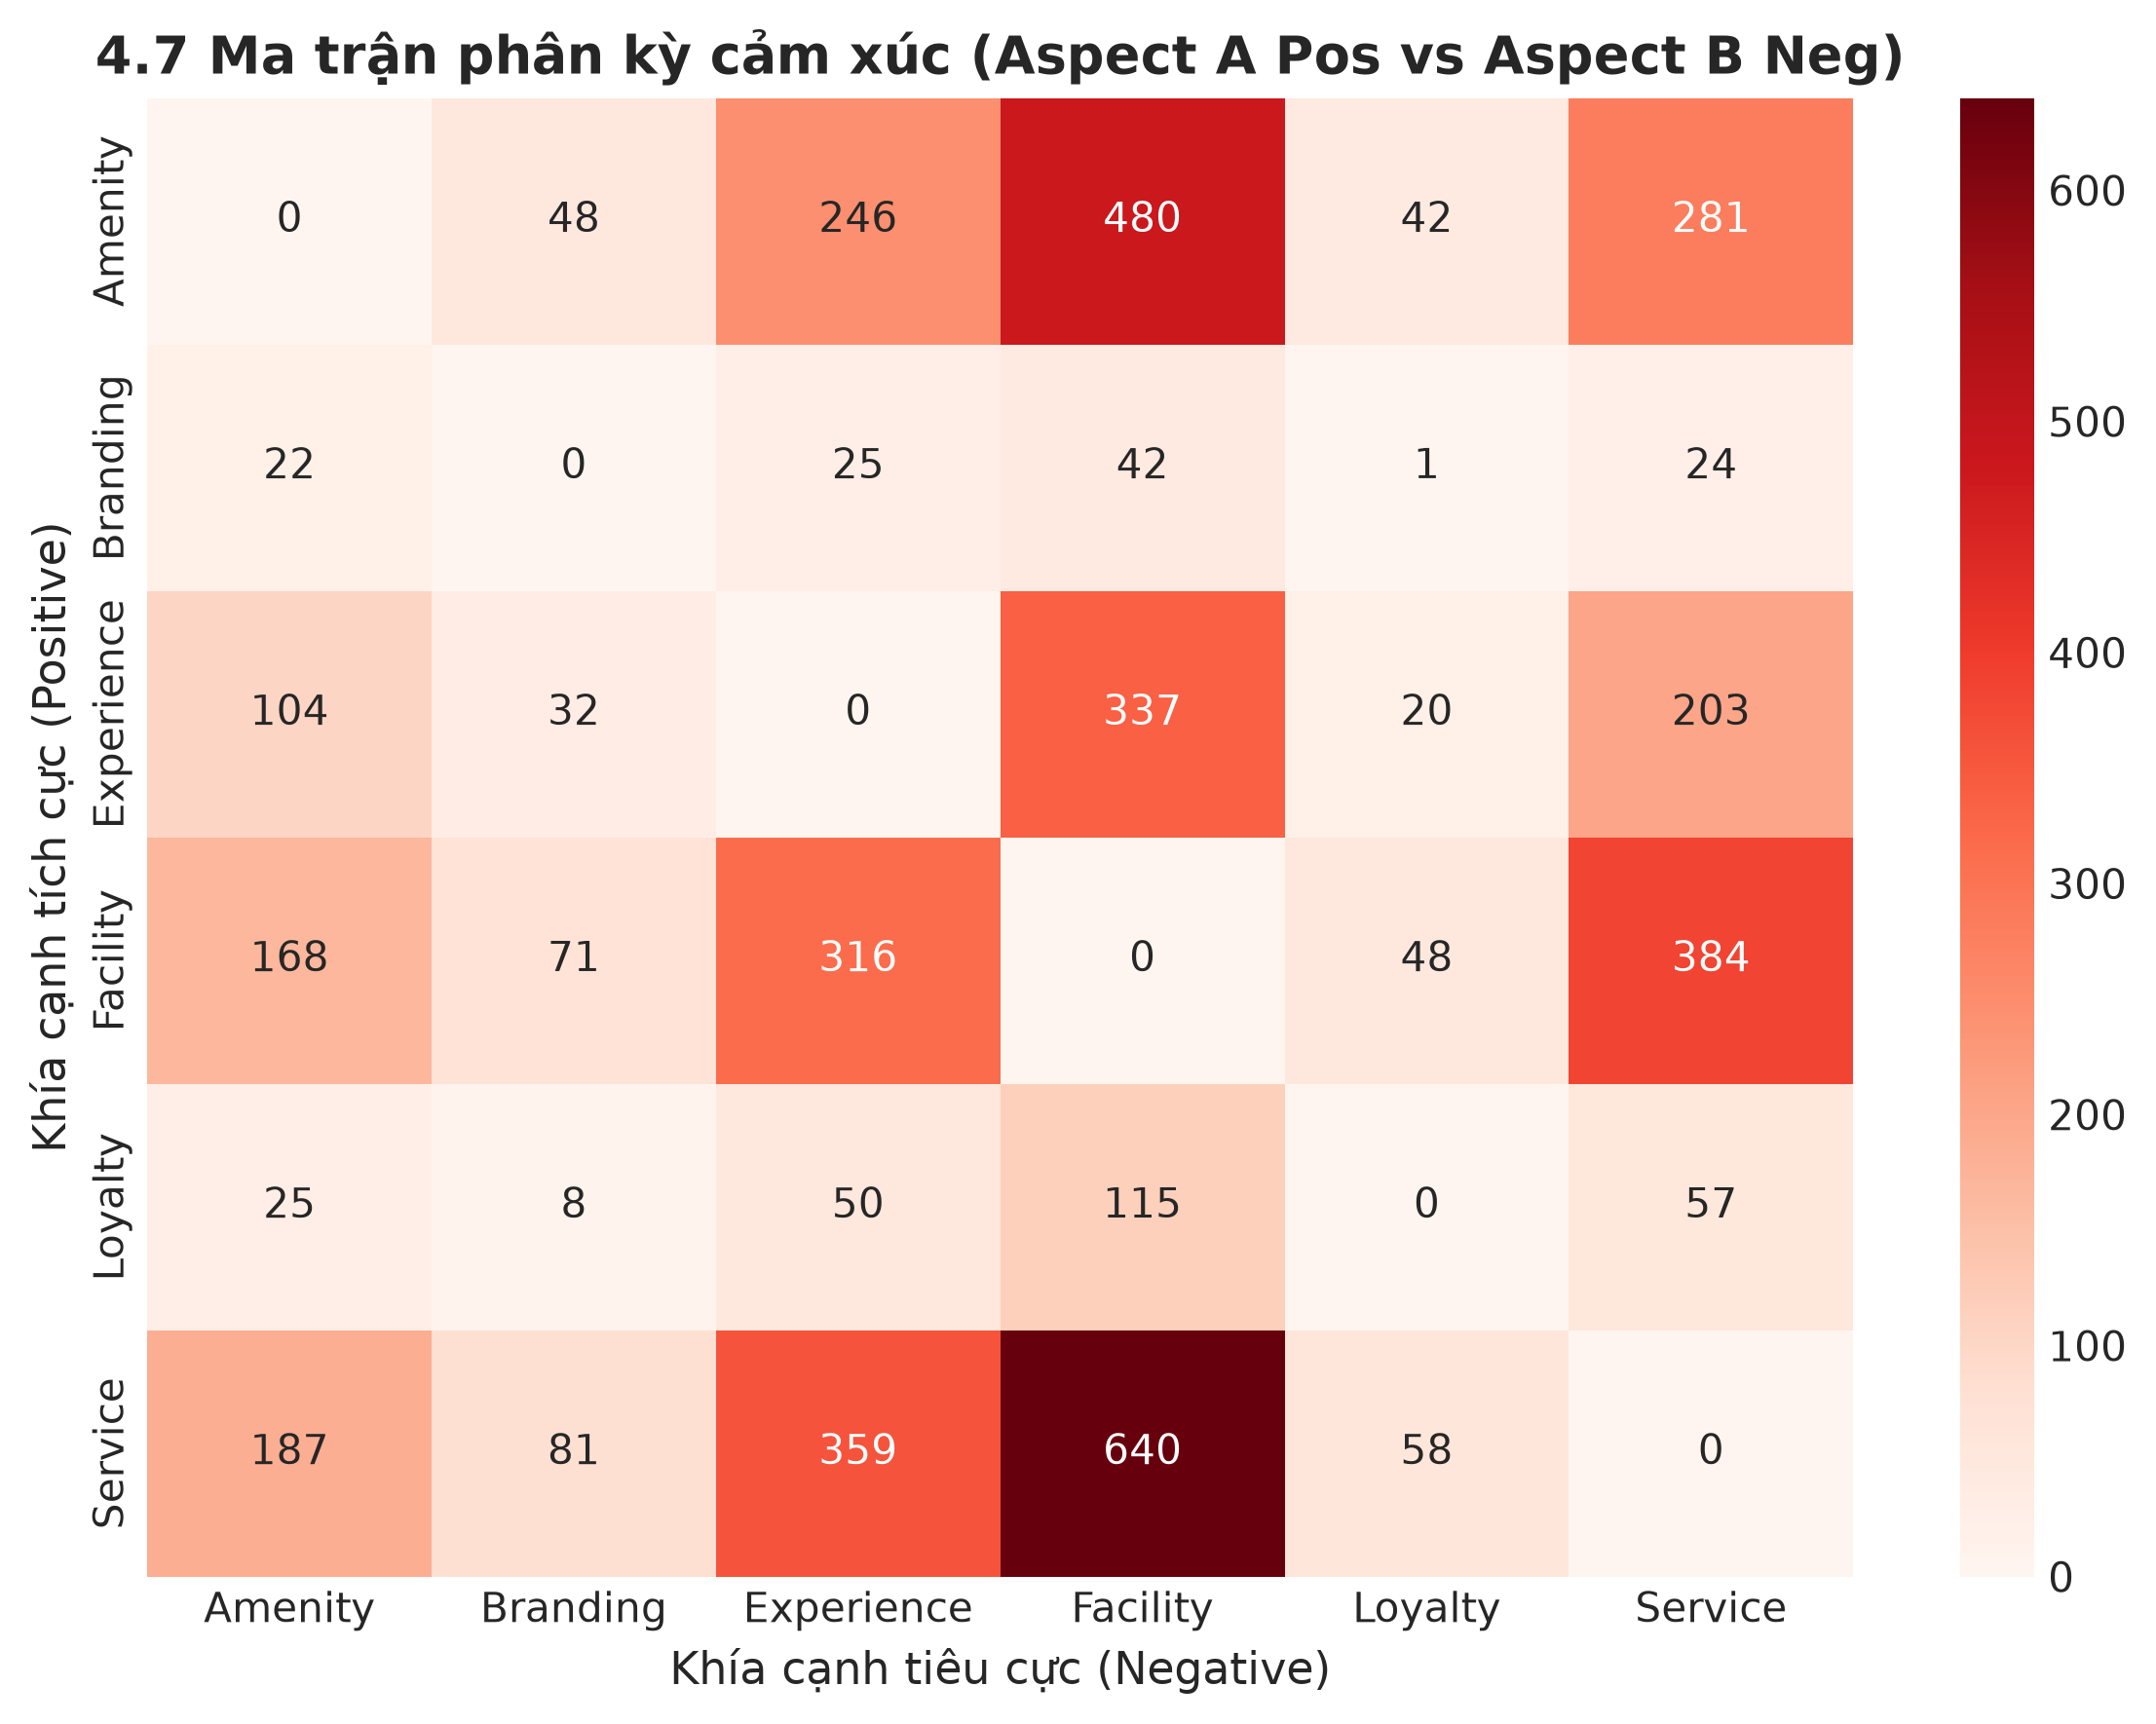
\includegraphics[width=\linewidth]{chart_img/47_sentiment_divergence_rate.png}
    \caption{Ma trận phân kỳ cảm xúc giữa các cặp khía cạnh (Aspect A Tích cực vs. Aspect B Tiêu cực), minh chứng trực quan cho hiện tượng ý kiến hai chiều đối lập (\textit{dual valences}) trong dữ liệu thực tế.}
    \label{fig:sentiment_divergence}
\end{figure}

Để minh chứng cho hiện tượng này trên dữ liệu thực nghiệm, Hình~\ref{fig:sentiment_divergence} thể hiện ma trận phân kỳ cảm xúc: trục dọc biểu thị các khía cạnh được khách hàng khen ngợi (Positive), còn trục ngang biểu thị các khía cạnh bị chê trách (Negative) trong cùng một bài đánh giá. Biểu đồ chỉ ra rằng sự phân kỳ xảy ra rất phổ biến giữa nhóm khía cạnh Cơ sở vật chất (\textit{Facility}), Trải nghiệm chung (\textit{Experience}) và Chất lượng dịch vụ (\textit{Service}). Điều này khẳng định rằng cảm xúc của du khách gắn liền với từng dịch vụ cụ thể là hoàn toàn độc lập, đòi hỏi bài toán phải bóc tách cảm xúc ở cấp độ khía cạnh riêng biệt.

Để giải quyết vấn đề trên, nghiên cứu tập trung vào sáu khía cạnh chính của chatbot, gồm \textit{Service}, \textit{Facility}, \textit{Experience}, \textit{Amenity}, \textit{Loyalty} và \textit{Branding}. Mỗi khía cạnh cần được liên kết với đoạn văn bản phù hợp trong bài đánh giá. Chẳng hạn, nhận xét về thái độ nhân viên cần được sử dụng làm bằng chứng cho khía cạnh dịch vụ, trong khi nhận xét về độ sạch sẽ của phòng cần được gắn với khía cạnh tương ứng.

Để thực hiện điều này một cách chuẩn xác, việc phân rã bài đánh giá thành các phân đoạn câu (sentence segments) là điều kiện tiên quyết, tương tự như quy trình được Nawawi và cộng sự~\cite{nawawi2024exploring} đề xuất: ``\textit{the research framework involves keyword extraction, sentence segment detection, aspect construction, and sentiment polarity measurement... Each identified segment, along with its corresponding keywords, was then subjected to sentiment polarity measurement}''~\cite{nawawi2024exploring}. Dựa trên định hướng này, bài toán trong nghiên cứu không chỉ là xác định cảm xúc mà còn là tìm đúng đoạn văn bản làm bằng chứng độc lập cho từng khía cạnh.

\begin{figure}[H]
    \centering
    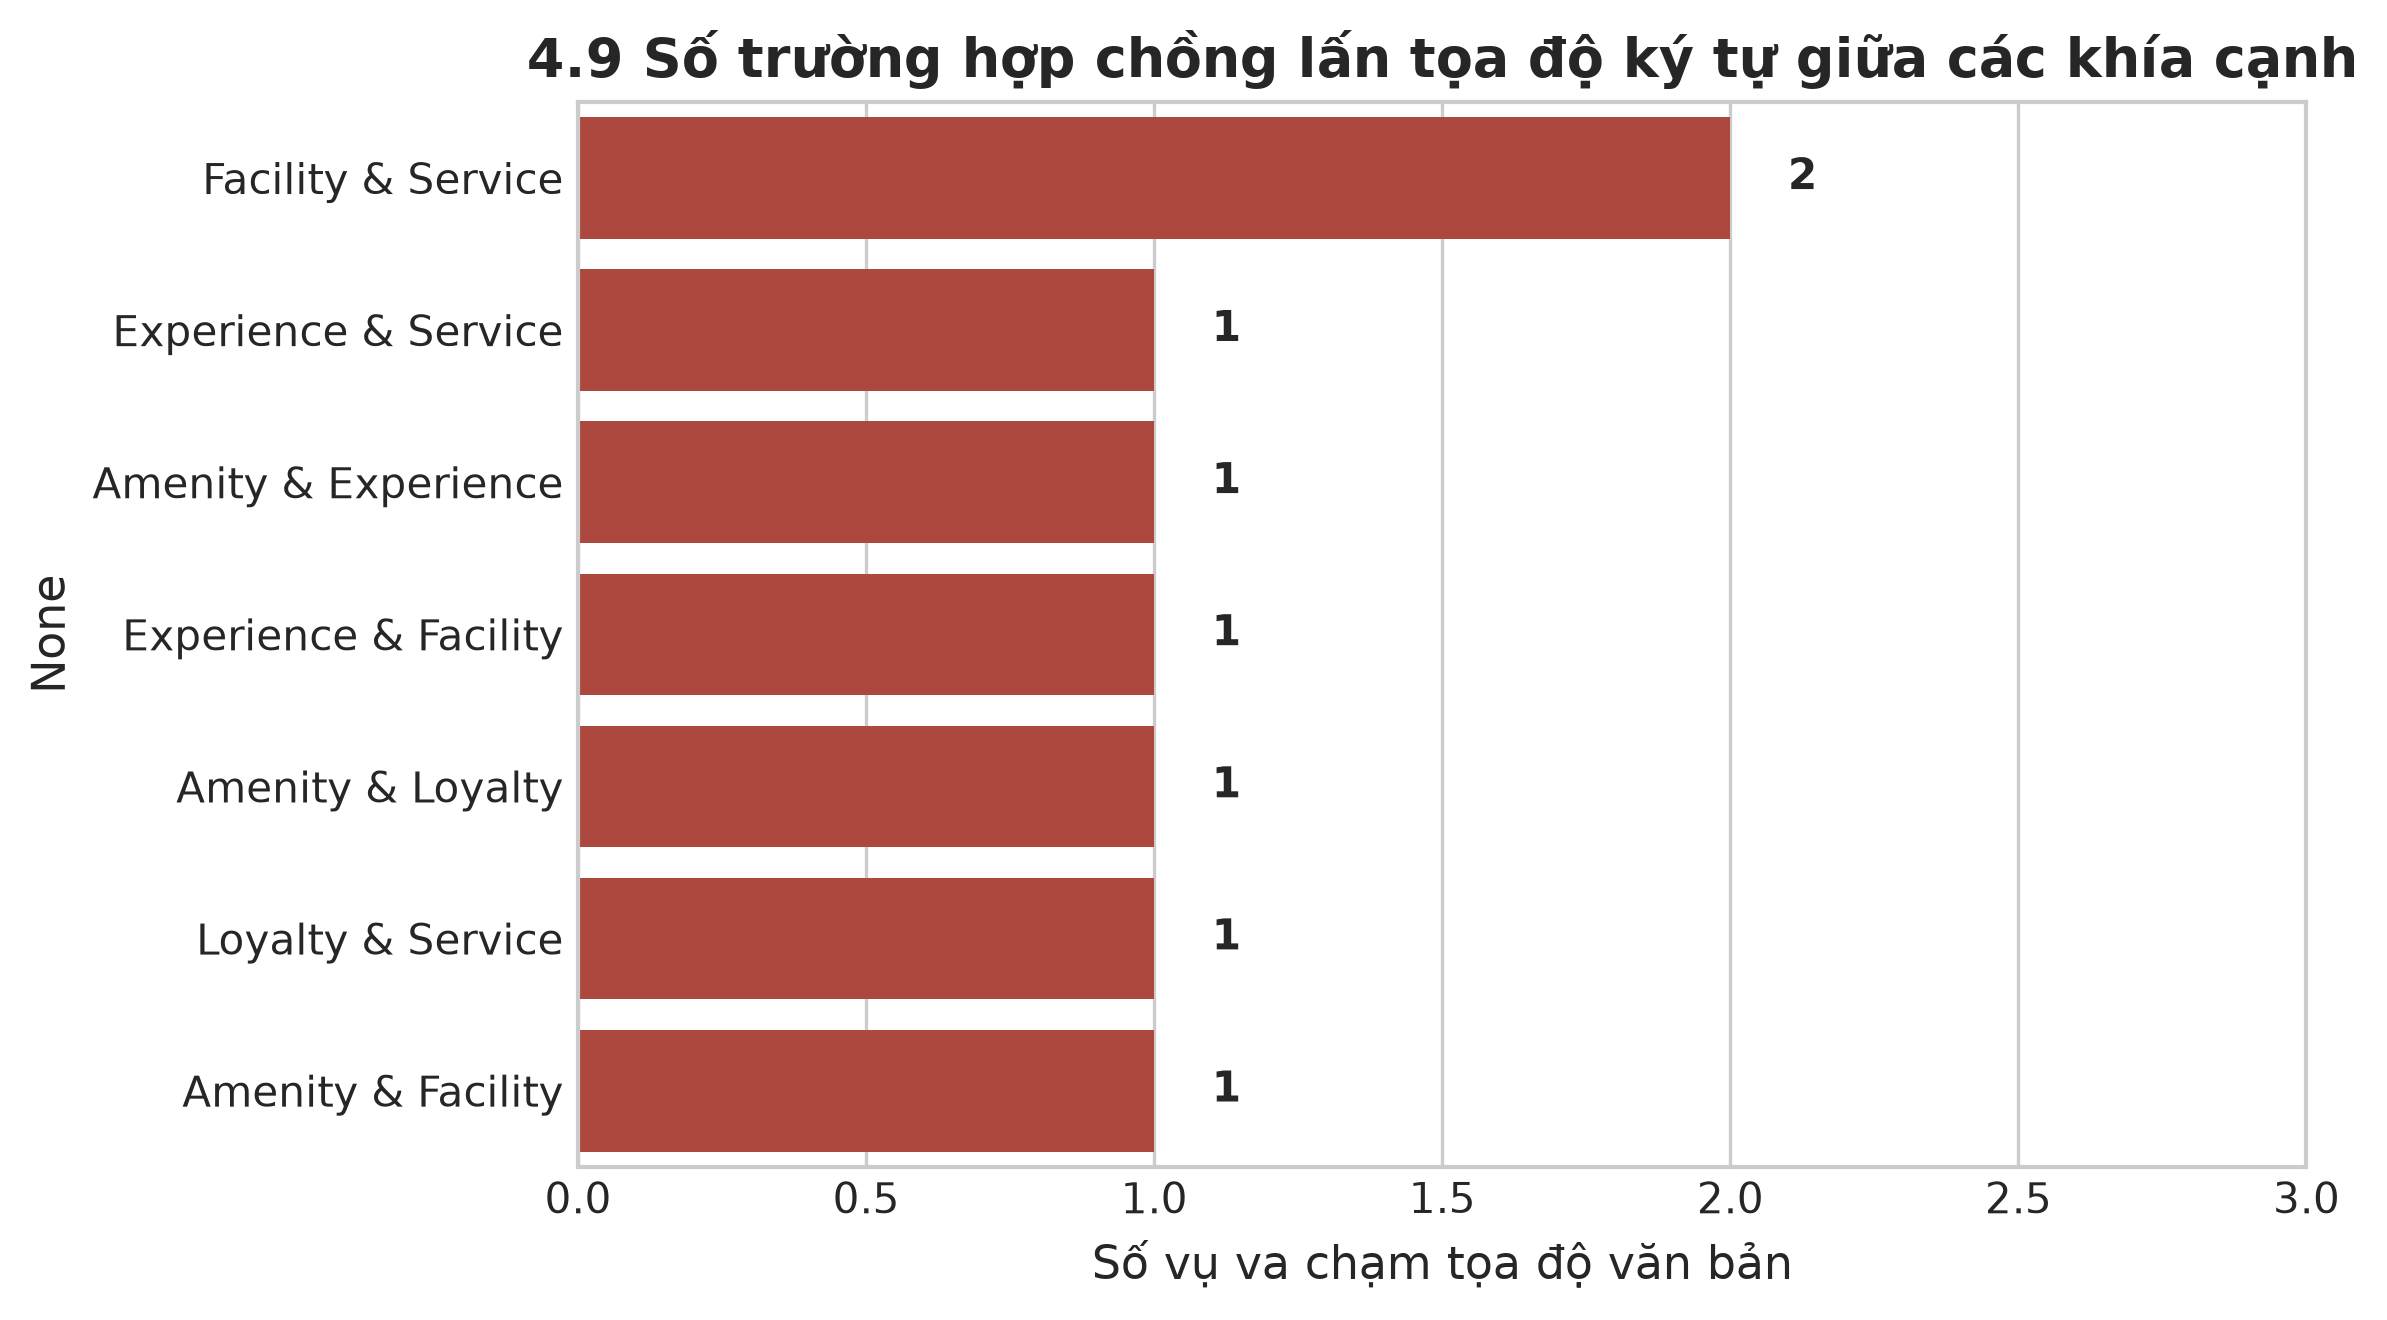
\includegraphics[width=\linewidth]{chart_img/49_cross_aspect_span_overlap.png}
    \caption{Thống kê số trường hợp chồng lấn tọa độ văn bản (bằng chứng) giữa các cặp khía cạnh, minh họa thách thức rò rỉ và lẫn bằng chứng (\textit{cross-aspect rationale leakage}).}
    \label{fig:span_overlap}
\end{figure}

Tuy nhiên, trong văn bản thực tế, người dùng thường viết các câu phức hợp nối liền nhau, dẫn đến hiện tượng chồng lấn tọa độ ký tự (span overlap) giữa các đoạn bằng chứng. Như minh họa tại Hình~\ref{fig:span_overlap}, dữ liệu ghi nhận hàng trăm trường hợp ranh giới văn bản giữa các khía cạnh (đặc biệt là giữa \textit{Facility} và \textit{Service}) bị trùng đè lên nhau. Hậu quả thực tế là nếu mô hình AI không được ràng buộc chặt chẽ, hiện tượng rò rỉ bằng chứng liên khía cạnh (\textit{cross-aspect rationale leakage}) sẽ xảy ra: mô hình có thể lấy nhầm một câu khen về phòng ngủ tiện nghi để trả lời cho câu hỏi của người dùng về thái độ phục vụ của nhân viên lễ tân. Đây là một sai sót nghiêm trọng làm giảm tính minh bạch và độ tin cậy của chatbot. Vì vậy, số liệu thực nghiệm từ Hình~\ref{fig:span_overlap} chính là cơ sở cốt lõi để nghiên cứu thiết kế cơ chế phạt chồng lấn phân đoạn ($\mathcal{L}_{\text{overlap}}$) trong khung CRAM-ABSA nhằm ép các vùng bằng chứng phải hoàn toàn tách biệt.


\subsubsection{Hỏi đáp khách sạn dựa trên bằng chứng}

Các kết quả phân tích được sử dụng để hỗ trợ chatbot trả lời câu hỏi liên quan đến khách sạn. Khi người dùng đặt câu hỏi, hệ thống cần xác định khách sạn được quan tâm, khía cạnh cần tìm hiểu và nội dung thông tin mà người dùng muốn biết. Sau đó, chatbot tìm kiếm những đánh giá phù hợp và sử dụng các đoạn bằng chứng liên quan để tạo câu trả lời.

Việc kết hợp nội dung văn bản với siêu dữ liệu (metadata) giải quyết hạn chế lớn của các mô hình hỏi đáp truyền thống, như Bruni và cộng sự~\cite{bruni2025amaqa} đã khẳng định: ``\textit{Retrieval-augmented generation (RAG) systems are widely used in question-answering (QA) tasks, but current benchmarks lack metadata integration, limiting their effectiveness in domain-specific scenarios}''~\cite{bruni2025amaqa}. Trong bài toán của chúng tôi, các thông tin như tên khách sạn, khía cạnh đánh giá và thời gian đăng bài được sử dụng để thu hẹp không gian tìm kiếm trước khi tổng hợp câu trả lời.

Ví dụ, khi người dùng hỏi về chất lượng bữa sáng hoặc thái độ phục vụ của nhân viên, chatbot cần ưu tiên những đánh giá liên quan trực tiếp đến nội dung đó thay vì đưa ra nhận xét chung chung về khách sạn. Câu trả lời cần ngắn gọn, dễ hiểu và có căn cứ từ dữ liệu. Nếu không tìm thấy đủ bằng chứng phù hợp, hệ thống cần thể hiện rõ giới hạn thông tin thay vì tự đưa ra kết luận không được hỗ trợ bởi các bài đánh giá.

Thông tin thời gian cũng đóng vai trò quyết định khi người dùng muốn tìm hiểu về chất lượng dịch vụ gần đây. Thay vì giả định chất lượng dịch vụ là cố định, Yu và cộng sự~\cite{yu2024dynamic} đã chứng minh rằng: ``\textit{The results indicate that the hotel attributes that consumers care about (e.g., Clean, Breakfast, and Front Desk) are dynamically fluctuating, and the attention and satisfaction of corresponding attributes will also change... it is particularly important to classify service quality attributes from a dynamic perspective}''~\cite{yu2024dynamic}. Đồng thời, việc phân tích mốc thời gian đăng bài như phương pháp của Nakamura và Oomiya~\cite{nakamura2021applying} giúp theo dõi sự dịch chuyển thực tế trong dịch vụ của khách sạn qua từng giai đoạn. Do đó, trong trường hợp dữ liệu có ngày đăng hợp lệ, những đánh giá mới hơn sẽ được ưu tiên trong quá trình truy xuất để phản ánh đúng hiện trạng, trong khi vẫn lưu giữ các đánh giá cũ để tái hiện bức tranh trải nghiệm dài hạn của khách sạn.

Tóm lại, bài toán của nghiên cứu là kết hợp việc trích xuất bằng chứng, phân tích cảm xúc theo khía cạnh và dự đoán điểm đánh giá để hỗ trợ chatbot hỏi đáp về khách sạn. Hệ thống hướng đến việc cung cấp câu trả lời đúng trọng tâm, hạn chế nhầm lẫn giữa các khía cạnh và sử dụng những nhận xét thực tế làm căn cứ. Phần tiếp theo sẽ trình bày phương pháp đề xuất CRAM-ABSA và cách các thành phần của mô hình được thiết kế để giải quyết những vấn đề trên.


\subsection{Phương pháp đề xuất - Proposed method}
\label{subsec:proposedmethod}

...

\subsection{Thiết lập thực nghiệm - Experimental}
\label{subsec:experimental}

...

\subsection{Tiêu chí đánh giá - Evaluation}
\label{subsec:evaluation}

...


%========================================================
% 3. Result & Discussion
%========================================================
\section{Result \& Discussion}
\label{sec:resultanddiscussion}
...

%========================================================
% 4. Conclusion
%========================================================
\section{Conclusion}
\label{sec:conclusion}
...

%========================================================
% 5. RESEARCH PLAN
%========================================================
\section{Research Plan}
\label{sec:plan}



%========================================================
% REFERENCES
%========================================================


\begin{thebibliography}{99}
    
    \bibitem[1]{bimaputra2023aspect}
    Bimaputra, D. S., \& Sutoyo, E.
    Aspect-Based Sentiment Analysis of Hotels in Bali on Tripadvisor Using BERT Algorithm.
    \textit{International Journal of Advances in Data and Information Systems}, 4(1), 29--40 (2023).
    DOI: \url{https://doi.org/10.25008/ijadis.v4i2.1284}
    
    \bibitem[2]{bruni2025amaqa}
    Bruni, D., Avvenuti, M., Tonellotto, N., \& Tesconi, M.
    AMAQA: A Metadata-based QA Dataset for RAG Systems.
    \textit{arXiv preprint arXiv:2505.13557} (2025).
    DOI: \url{https://doi.org/10.48550/arXiv.2505.13557}
    
    \bibitem[3]{nakamura2021applying}
    Nakamura, Y., \& Oomiya, N.
    Applying the Topic Model to Hotel Reviews of Internet Sites and Analyzing Their Results.
    \textit{Journal of Global Tourism Research}, 6(1), 15--20 (2021).
    DOI: \url{https://doi.org/10.37020/jgtr.6.1_15}
    
    \bibitem[4]{namee2023hybrid}
    Namee, K., Polpinij, J., \& Luaphol, B.
    A Hybrid Approach for Aspect-based Sentiment Analysis: A Case Study of Hotel Reviews.
    \textit{Current Applied Science and Technology}, 23(2), 1--16 (2023).
    DOI: \url{https://doi.org/10.55003/cast.2022.02.23.008}
    
    \bibitem[5]{nawawi2024exploring}
    Nawawi, I., Ilmawan, K. F., Maarif, M. R., \& Syafrudin, M.
    Exploring Tourist Experience through Online Reviews Using Aspect-Based Sentiment Analysis with Zero-Shot Learning for Hospitality Service Enhancement.
    \textit{Information}, 15(8), 499 (2024).
    DOI: \url{https://doi.org/10.3390/info15080499}
    
    \bibitem[6]{yu2024dynamic}
    Yu, W., Cui, F., Wang, P., \& Liao, X.
    Dynamic Mining of Consumer Demand via Online Hotel Reviews: A Hybrid Method.
    \textit{Journal of Theoretical and Applied Electronic Commerce Research}, 19(3), 1831--1847 (2024).
    DOI: \url{https://doi.org/10.3390/jtaer19030090}
    
    \bibitem[32]{tran2026aspect}
    Tran, T. K., \& Tran, P.
    Aspect-based Sentiment Analysis in Ho Chi Minh city Hotel Reviews using Aspect-Conditioned BiLSTM with Cross-Aspect Attention and Ordinal Regression.
    \textit{IEEE Access}, 14, 1--15 (2026).
    DOI: \url{https://doi.org/10.1109/ACCESS.2026.3671083}
    
\end{thebibliography}

\end{document}
